\documentclass[Ex4_Zusammenfassung.tex]{subfiles}
\begin{document}

\chapter{Strukturinformation aus Streuexperimenten}
\textbf{von \martina} \\ 
 
\textbf{Definition Struktur:} 
Räumliche Verteilung von Masse,Ladung und Magnetisierung  \\ \newline 
Um etwas über die räumliche Struktur zu erfahren, misst man den Wirkungsquerschnitt (Streuwahrscheinlichkeit in Form einer Fläche) in Abhängigkeit vom Streuwinkel (der mit dem Impulsübertrag zusammenhängt). \newline

\section{Elastische Streuung}
\subsection{Rutherford-Streuung}
$\alpha$-Teilchen streuen an einer Goldfolie. Dieses Experiment führte zur Entdeckung der Atomkerne. \newline
\textbf{Annahme über Streupartner:} punktförmig, geladen, $E_{kin} \ll$ Masse \newline
Rutherford fand für den differentiellen Wirkungsquerschnitt pro Raumwinkel von Teilchen mit Ladungszahl z der kinetischen Energie T welche unter dem Winkel $\theta$  an Teilchen der Kernladungszahl Z streuen folgende Beziehung:
\begin{equation}
\frac{d\sigma^R}{d\Omega} = \frac{(zZe^2)^2}{16T^2 \text{sin}^4 (\theta/2)}
\end{equation}
Die Messungen zeigten, dass der Atomkern kleiner ist als die Annäherung der $\alpha$-Teilchen.
Es gilt Energieerhaltung:
\begin{equation}
T = \frac{mv'^2}{2} + \frac{zZe^2}{\delta_{min}}
\end{equation}
Wobei v' die Geschwindigkeit des abgelenkten Teilchens nach der Streuung ist (siehe Abb.7.1).

\begin{figure}[h]
\centering
	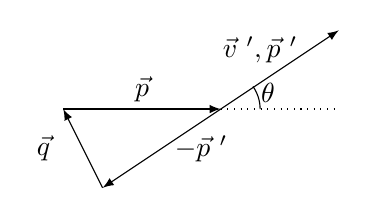
\begin{tikzpicture}
	\draw[->, -latex] (0,0) -- (2,0);
	\draw[->, -latex] (2,0) -- (0.5,-1);
	\draw[->, -latex] (0.5,-1) -- (0,0);
	\draw [dotted] (2,0) -- (3.5,0);
	\draw[->, -latex] (2,0) -- (3.5,1);
	\draw (2.5,0) arc(0:35:0.5cm);
	
	\node at (1,0.25) {$  \vec p$};
	\node at (2.5,0.75) {$\vec v \ ' ,  \vec p \ '$};
	\node at (1.75,-0.5) {$ - \vec p \ '$};
	\node at (-0.25,-0.5) {$ \vec q$};
	\node at (2.6,0.2) {$\theta$};
	\end{tikzpicture}
	\caption{Impulse bei Streuung}
\end{figure}
Die größtmögliche Annäherung bei Rückwärtsstreuung ($\theta=$180°) erhält man mit v'= 0 zu: 
\begin{equation}
\delta_{min} = \frac{zZe^2}{T}
\end{equation}
Mit Abb. 7.1 lässt sich auch gut der Impulsübertrag $\vec q$ berechnen zu: 
\begin{align}
\vec q &= \vec p - \vec p \ ' \\
|\vec q| &= 2 \  |\vec p| \  \text{sin}(\theta/2)
\end{align} 
Dieser ist nicht zu verwechseln mit dem Viererimpulsübertrag: 
\begin{equation}
q^2 = (E-E')^2 - |\vec q|^2
\end{equation}
Es ist zweckmäßig den differentiellen Wirkungsquerschnitt durch eine Streuamplitude zu beschreiben:
\begin{equation}
\frac{d\sigma}{d\Omega} = |f(\vec q^2)|^2
\end{equation}
Im Falle einer Streuung eines Teilchens an einem kugelsymmetrischen Coulomb-Potential eines Kerns wird das Teilchen durch eine ebene Welle beschrieben. Die Ebene wird durch das Skalarprodukt $ \vec p \cdot \vec r $ beschrieben.
\begin{equation}
\psi_j = \text{exp} \left(\frac{i \vec p \cdot \vec r}{\hslash}\right)
\end{equation}
Die Streuamplitude erhält man nun durch Fouriertransformation des Potentials des Kerns V(r) in den Impulsraum welcher durch den Impulsübertrag $ \vec q^2 $ beschrieben wird. Wir definieren $ q = |\vec q|$ und $ r = |\vec r|$
\begin{align}
f(\vec q \ ^2) &= -\frac{m}{2\pi \hslash^2} \int V(r) \  \text{exp} \left(\frac{i \vec p \cdot \vec r}{\hslash}\right) d \vec r \\
&= -\frac{2m}{q\hslash^2} \int r \  V(r) \  \text{sin} \left(\frac{qr}{r}\right) d\vec r
\end{align} 
 Man kann sich eine Zerlegung der Streuamplitude in Elementarwellen $\text{exp} \left(\frac{i \vec p \cdot \vec r}{\hslash}\right)$  vorstellen, mit dem Gewichtungsfaktor des Potentials am Ort $\vec r$. Man stellt sich also die Streuamplitude als Amplitude der Superposition aller Wellenfronten  $\text{exp} \left(\frac{i \vec p \cdot \vec r}{\hslash}\right)$ vor, wobei eine einzelne Wellenfront stärker/schwächer ins Gewicht fällt, wenn das Potential V(r) an dem Ort $\vec r$ größer/kleiner ist. Dies ist plausibel, da falls das Potential V(r) groß/klein ist, die Streuwahrscheinlichkeit auch größer/kleiner ist. Somit sollte die Streuamplitude, welche die Streuwahrscheinlichkeit beschreibt, mit dem Potential V(r) skalieren. \newline
 Berücksichtigt man die Abschirmung des Potentials von Elektronen so erhält man als Potential
 \begin{equation}
 V(r)=\frac{zZe^2}{r} e^{-\nicefrac{r}{a}} 
 \end{equation}
 mit dem Skalierungsfaktor $a\approx 1  \text{\AA}$ \newline
 Somit erhalten wir als differentiellen Wirkungsquerschnitt 
\begin{equation}
\frac{d\sigma}{d\Omega} = |f(q^2)|^2 = \frac{4m^2z^2Z^2e^4}{q^4}
\end{equation}
Für relativistische Teilchen kann $E\approx p $ angenommen werden. Wir erhalten hier als Wirkungsquerschnitt pro Impulsübertrag
\begin{equation}
\frac{d\sigma}{d(q^2)} = \frac{d\sigma}{d\Omega} \frac{d\Omega}{d(q^2)} = \frac{4 \pi(zZ)^2e^4}{q^4}
\end{equation}
Im Laborsystem muss bei relativistischen Teilchen der Rückstoß berücksichtigt werden
\begin{align}
\frac{d\sigma}{d(q^2)} &= \frac{d\sigma}{d(q^2_{cms})} \frac{E'}{E} \\
\frac{E'}{E} &= \frac{1}{1+\frac{2E}{m} \text{sin}^2(\frac{\theta}{2})}
\end{align}

\subsection{Streuung relativistischer Spin \nicefrac{1}{2}-Teilchen an Punktladung Ze}
Berücksichtigt man den Spins eines Teilchens, so muss man das durch den Spin hervorgerufene Magnetische Moment bei Streubetrachtungen hinzuziehen. Dadurch erhält man den \textbf{Mott-Querschnitt}
\begin{equation}
\derive{\sigma^M}{(q^2)} = \frac{4 \pi Z^2 e^4}{q^4}\left(1-\beta^2 \sin^2 \left(\frac{\theta}{2}\right)\right)
\end{equation} \newpage

\subsection{Streuung an ausgedehnter Ladungsverteilung}
Für das Potential gilt die Poisson-Gleichung
\begin{equation}
- \nabla^2 V = 4 \pi \rho(r) Ze^2
\end{equation}
Unter Verwendung einer Green'schen Identität lässt sich das Integral für die Streuamplitude umschreiben 
\begin{equation}
\int \md \vec r \  \text{exp} \left(i \frac{ \vec q \cdot \vec r }{\hslash} \right) V(r) = - \frac{\hslash^2}{q^2} \int \md \vec r \  \text{exp} \left(i \frac{\vec q \cdot \vec r }{\hslash}\right) \nabla^2 V(r)
\end{equation}
Und man erhält als differentiellen Wirkungsquerschnitt:
\begin{equation}
\derive{\sigma}{\Omega} = |f(q^2)|^2 = \frac{4m^2Z^2e^4}{q^4} \left|\int \md \vec r \  \text{exp}\left(i \frac{ \vec q \cdot \vec r }{\hslash} \right) \rho(r)  \right|^2
\end{equation}
Das letzte Integral hat eine wichtige Bedeutung, weshalb man es als den Formfaktor definiert. Dieser ist die Fouriertransformierte der Ladungsverteilung und enthält die ganze Streuinformation des Wirkungsquerschnitts.
\begin{equation}
F(q^2) = \int \md \vec r \   \text{exp}\left(i \frac{ \vec q \cdot \vec r }{\hslash} \right) \rho(r)
\end{equation}
Man kann damit den Wirkungsquerschnitt recht einfach aus dem Rutherford-Querschnitt erhalten:
\begin{equation}
\derive{\sigma}{\Omega} = \derive{\sigma^R}{\Omega} |F(q^2)|^2
\end{equation}
\end{document}